\documentclass[11pt]{article}
\usepackage{graphicx}
\usepackage{amsmath,textcomp,amssymb,geometry,graphicx,enumerate}
\usepackage{algorithm} % Boxes/formatting around algorithms
\usepackage[noend]{algpseudocode} % Algorithms
\usepackage{hyperref}
\usepackage{inconsolata}
\usepackage{subcaption}
\newtheorem{theorem}{Theorem}
\newtheorem{lemma}[theorem]{Lemma}
\hypersetup{
	colorlinks=true,
	linkcolor=blue,
	filecolor=magenta,      
	urlcolor=blue,
}

\title{EE660 -- Spring 2024 --- Homework 5}
\author{Altman (Gujia) Ma}
\date{}

\textheight=9in
\textwidth=6.5in
\topmargin=-.75in
\oddsidemargin=0.25in
\evensidemargin=0.25in


\begin{document}
	\maketitle
	
	Collaborators: n/a
	In this Homework, I will apply DSM and EBM on all generators. Also I tried VAE and DDPM, but met problems when doing training so I gave up. However, the jupyter notebooks for the failed trails are also submitted. 
	\section*{1. Denosing Score Mathinc Method}
	In this part, I applied DSM on all four of the generators. 
	The training process is recorded in four Jupyter notebooks:\\ Chekerbooks in \texttt{denoising\_score\_matching.ipynb}, PinWheel in \texttt{denoising\_score\_matching\_pin.ipynb}, Spiral in \texttt{denoising\_score\_matching\_Spin.ipynb} and Gaussian Mixtures in\\ \texttt{denoising\_score\_matching\_Gaussian.ipynb}. \\
	I applied the same superparameters for all four datasets:\\\texttt{
	The MLP has 2 hidden layers with 64 nerons on each layer, and 2 on output layer. \\
	Activation: Swish Function.\\
	Learning Rate: 0.001.\\
	Optimizer: Adam.\\
	Batch size: 128.\\
	Number of Epoches: 5000,\\
	Noise Level: 0.1.\\}
	The training losses while training process in four datasets are listed below.\\
	From the training losses functions, we can see that the training on Checker and Gaussian dataset goes very well: The loss keeps decreasing and get a low enough number. However, the cases is not as good in Spiral and PinWheel cases.
	\begin{figure}[H]
		\centering 
		\begin{subfigure}{0.45\textwidth}
			\centering
			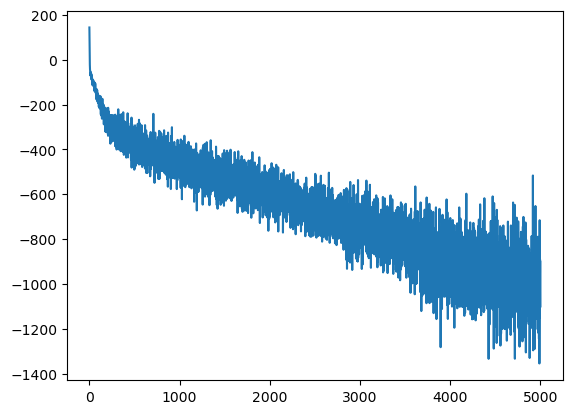
\includegraphics[width=\textwidth]{DSM_Checker_Loss.png}
			\caption{DSM training Loss function on Checker data}
			\label{fig:DSMChckerLoss}
		\end{subfigure}
		\hfill
		\begin{subfigure}{0.45\textwidth}
			\centering
			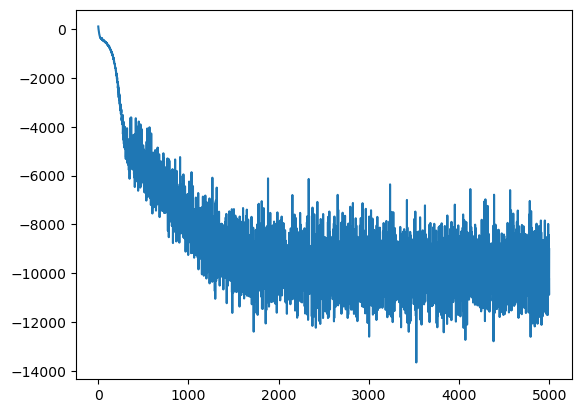
\includegraphics[width=\textwidth]{DSM_Gaussian_Loss.png}
			\caption{DSM training Loss function on Gaussian data}
			\label{fig:DSMGaussianLoss}
		\end{subfigure}
		\\
		\begin{subfigure}{0.45\textwidth}
			\centering
			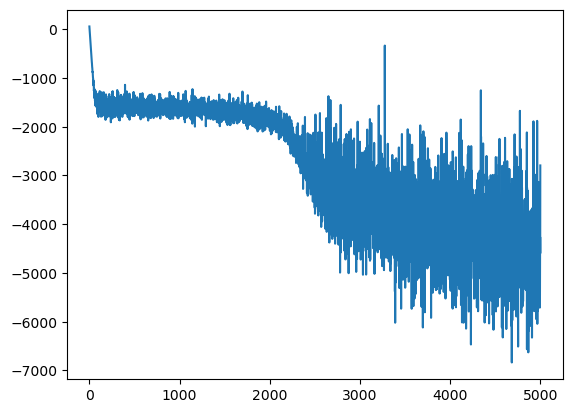
\includegraphics[width=\textwidth]{DSM_Pin_loss.png}
			\caption{DSM training Loss function on PinWheel data}
			\label{fig:DSMPinLoss}
		\end{subfigure}
		\hfill
		\begin{subfigure}{0.45\textwidth}
			\centering
			\includegraphics[width=\textwidth]{DSM_Spin_loss.png}
			\caption{DSM training Loss function on Spiral data}
			\label{fig:DSMSpinLoss}
		\end{subfigure}
		
		\caption{DSM training Losses}
		\label{DSMTLoss}
	\end{figure}
	\section*{2. Energy Based Model}
	In this part, I applied DSM on all four of the generators. 
	The training process is recorded in four Jupyter notebooks:\\ Chekerbooks in \texttt{EBM.ipynb}, PinWheel in \texttt{EBM\_pin.ipynb}, Spiral in \texttt{EBM\_Spin.ipynb} and Gaussian Mixtures in \texttt{EBM\_Gaussian.ipynb}. \\
	The super parameters are listed below:\\
	\\texttt{
		The MLP has 2 hidden layers with 64 nerons on each layer, and 2 on output layer. \\
		Activation: relu.\\
		Learning Rate: 0.001.\\
		Optimizer: Adam.\\
		Batch size: 128.\\
		Step size: 0.01.\\
		Number of Epoches: 5000,\\
		Noise Level: 0.1.\\}
	And the training losses are listed below. 
		\begin{figure}[H]
		\centering 
		\begin{subfigure}{0.45\textwidth}
			\centering
			\includegraphics[width=\textwidth]{EBM_Loss.png}
			\caption{BM training Loss function on Checker data}
			\label{fig:BMChckerLoss}
		\end{subfigure}
		\hfill
		\begin{subfigure}{0.45\textwidth}
			\centering
			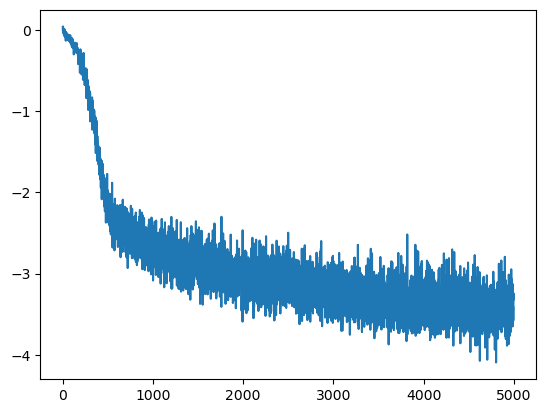
\includegraphics[width=\textwidth]{EBM_Gaussian_Loss.png}
			\caption{EBM training Loss function on Gaussian data}
			\label{fig:EBMGaussianLoss}
		\end{subfigure}
		\\
		\begin{subfigure}{0.45\textwidth}
			\centering
			\includegraphics[width=\textwidth]{EBM_Pin_loss.png}
			\caption{EBM training Loss function on PinWheel data}
			\label{fig:EBMPinLoss}
		\end{subfigure}
		\hfill
		\begin{subfigure}{0.45\textwidth}
			\centering
			\includegraphics[width=\textwidth]{EBM_Pin_loss.png}
			\caption{EBM training Loss function on Spiral data}
			\label{fig:EBMSpinLoss}
		\end{subfigure}
		
		\caption{EBM training Losses}
		\label{EBMTLoss}
	\end{figure}
	From the training losses, we can see that EBM fail to find a training path with decreasing training losses. The Training losses stopped decreasing at a very high level. 
	\section*{3. Qualitative comparison of model sample quality}
	The Comparison between Samples generated from the trained sample and from true distributions are shown below.
	\begin{figure}[H]
		\centering 
		\begin{subfigure}{0.45\textwidth}
			\centering
			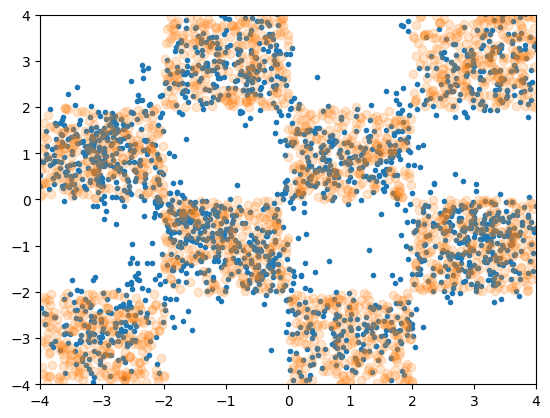
\includegraphics[width=\textwidth]{DSM_Checker.png}
			\caption{Samples from DSM traning model with Original Data}
			\label{fig:DSMChecker}
		\end{subfigure}
		\hfill
		\begin{subfigure}{0.45\textwidth}
			\centering
			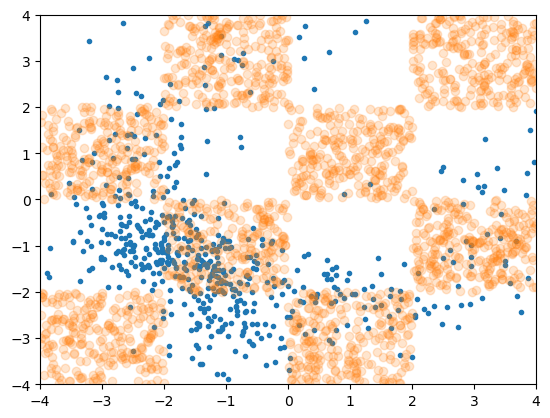
\includegraphics[width=\textwidth]{EBM.png}
			\caption{Samples from EBM traning model with Original Data}
			\label{fig:EBMChecker}
		\end{subfigure}
		\caption{Qualitative Comparison between DSM and EBM Models in Checker Dataset}
		\label{Chekcer}
	\end{figure}
\end{document}